\input{header}

\AtBeginSubsection[]
{
	\begin{frame}<beamer>
		\frametitle{Outline}
		\tableofcontents[current,currentsubsection]
	\end{frame}
}

\begin{document}

\begin{frame}[allowframebreaks]
\frametitle{Turing Machines:}
  \begin{itemize}
\item Part II: computability 
\item [] We would like to study
  problems that can  and cannot be solved by computers
\item We need a more powerful model

\item [] Finite automata: small memory (states)

\item [] PDA: unlimited memory (stack) by push/pop
\item Turing machine: unlimited and unrestricted memory

\item This is about everything a real computer can do

\item Thus problems not solved by Turing machines

\item [] $\Rightarrow$ beyond the limit of computation
\item A TM has a tape as the memory

\begin{center}
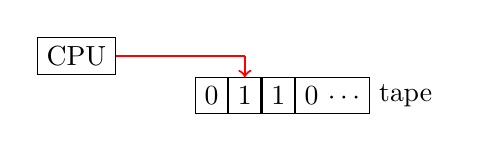
\begin{tikzpicture}[ampersand replacement=\&]
\matrix 
{
  \node[draw](0) {CPU}; \& [1cm] \& \node(1){}; \&\&\& \\
  \& \node[draw]{0}; \& \node[draw](a){1}; \& \node[draw]{1}; \& \node[draw]{0 $\cdots$};  \& \node{tape};\\
};
\draw [-,red,thick] (0) -- (1.center) ;
\draw [->,red,thick] (1.center) -- (a) ;
\end{tikzpicture}
\end{center}


\item Differences from finite automata
  \begin{itemize}
  \item write/read tape
  \item head moves left/right
  \item infinite space in the tape
  \item rejecting/accepting take immediate effect

  \item machine goes on forever, otherwise
  \end{itemize}
\item Example

  \begin{equation*}
B=\{w\#w\mid w \in \{0,1\}^*\}
\end{equation*}
\item We can prove that $B$ is not CFL using pumping lemma for CFL (similar to example 2.38)

\item Running a sample input. Figure 3.2
\item $\sqcup$: blank symbol
\item [] We assume infinite $\sqcup$'s after the input sequence
\item Strategy: zig-zag to the corresponding places on the two sides of the \# and determine
  whether they match.
  
\begin{center}
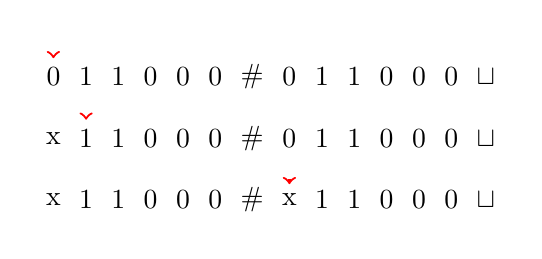
\begin{tikzpicture}[ampersand replacement=\&]
\matrix 
{
  \node(0){};  \&\&\&\&\&\& \& \&\&\&\&\&\& \\
  \node(01){0}; \& \node{1}; \& \node{1}; \& \node{0}; \& \node{0}; \&\node{0}; \&
  \node{\#}; \& 
  \node{0}; \& \node{1}; \& \node{1}; \& \node{0}; \& \node{0}; \& \node{0}; \& \node{$\sqcup$}; \\
    \& \node(1){};  \&\&\&\&\& \& \&\&\&\&\&\& \\
  \node{x}; \& \node(11){1}; \& \node{1}; \& \node{0}; \& \node{0}; \&\node{0}; \&
  \node{\#}; \& 
  \node{0}; \& \node{1}; \& \node{1}; \& \node{0}; \& \node{0}; \& \node{0}; \& \node{$\sqcup$}; \\
\&\&\&\&\&\& \&    \node(2){};   \&\&\&\&\&\& \\
  \node{x}; \& \node{1}; \& \node{1}; \& \node{0}; \& \node{0}; \&\node{0}; \&
  \node{\#}; \& 
  \node(21){x}; \& \node{1}; \& \node{1}; \& \node{0}; \& \node{0}; \& \node{0}; \& \node{$\sqcup$}; \\
};
\draw [->,red,thick] (0) -- (01) ;
\draw [->,red,thick] (1) -- (11) ;
 \draw [->,red,thick] (2) -- (21) ;
% \draw [->,red,thick] (1.center) -- (a) ;
\end{tikzpicture}
\end{center}



\item Algorithm:
  \begin{enumerate}
  \item scan to check \#
  \item check $w$ and $w$
  \end{enumerate}

\end{itemize}
\end{frame}

\begin{frame}[allowframebreaks] \frametitle{Formal definition of TM}
  \begin{itemize}
\item It's complicated and seldom used
\item $\delta$:
  \begin{equation*}
  Q\times \Gamma\rightarrow 
Q\times \Gamma \times\{L,R\}
\end{equation*}
\item Example:
  \begin{equation*}
  \delta(q,a) = (r,b,L)
\end{equation*}
\item [] $q$: current state

\item [] $a$: pointed in tape

\item [] $r$: next state

\item [] $b$: replace $a$ with $b$
\item [] $L$: head then moved to the left
\item $(Q,\Sigma, \Gamma, \delta, q_0, q_{accept},
q_{reject})$

\item [] $Q$: states

\item [] $\Sigma$: input alphabet (blank: $\sqcup \notin \Sigma$)

\item [] $\Gamma$: tape alphabet, $\sqcup \in \Gamma, 
\Sigma \subset \Gamma$

\item [] $\delta$:
  \begin{equation*}
  Q\times \Gamma \rightarrow
Q \times \Gamma \times 
\{L,R\}
\end{equation*}
\item [] $q_0 \in Q$, start

\item [] $q_{accept} \in Q$

\item [] $q_{reject} \in Q, q_{reject} \neq q_{accept}$

\item [] Single $q_{accept}, q_{reject}$

\item The input
  \begin{equation*}
  w_1\cdots w_n
\end{equation*}
is put in 
  positions $1 \ldots, n$ of the tape in the beginning

\item [] Assume $\sqcup$ in all the rest of the tape
\item If head points to first position and
    \begin{equation*}
  \delta(q,?) = (r,?,L)
\end{equation*}
then the head stays at the same position
\begin{center}
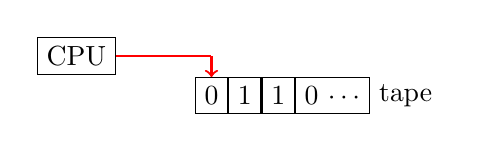
\begin{tikzpicture}[ampersand replacement=\&]
\matrix 
{
  \node[draw](0) {CPU}; \&  [1cm] \node(1){}; \&  \&\&\& \\
  \& \node[draw](a){0}; \& \node[draw]{1}; \& \node[draw]{1}; \& \node[draw]{0 $\cdots$};  \& \node{tape};\\
};
\draw [-,red,thick] (0) -- (1.center) ;
\draw [->,red,thick] (1.center) -- (a) ;
\end{tikzpicture}
\end{center}

\end{itemize}\end{frame}

\end{document}
